\documentclass[a4paper, 12pt]{article}
\usepackage[francais]{babel}
\usepackage{graphicx}
\usepackage[utf8]{inputenc}
\usepackage[T1]{fontenc}
\usepackage{fancyhdr}
\usepackage[margin=1in]{geometry}
\usepackage{amsmath}
\usepackage{amssymb}
\author{Thibault \bsc{BEZIERS LA FOSSE}}
\date{}
\title{Étude et Comparaison d'Algorithmes}



\pagestyle{fancy}
\begin{document}

\maketitle
\clearpage

\tableofcontents
\clearpage

\section{Introduction}
Ce projet en six séances à pour objectif d'implémenter des algorithmes, afin de calculer leurs complexités et comparer les performances. 
Quatre algorithmes sont à notre disposition, ce compte rendu les traitera dans l'ordre donné. Seront expliqués:
\begin{itemize}
\item[L'implémentation]
\item[La complexité théorique]
\item[Les résultats d'exécutions]
\item[L'analyse des résultats]
\item[Le comparatif des résultats théoriques et expérimentaux]
\end{itemize}
\subsection{Objectif}
Les quatre algorithmes à implémenter consistent à trouver la suite de termes du tableau dont la somme est maximum. 
Les éléments du tableau sont choisis de manière aléatoire, et nous exécuterons nos algorithmes sur des tableaux de tailles variables, en commençant par des tableaux de moins d'une dizaine d'éléments, à des tableaux qui en contiennent des dizaines de milliers.  
\subsection{Outils utilisés}
Le langage de programmation à utiliser pour ce projet étant libre, j'ai choisi de m'orienter vers le C++. D'abord pour une raison pratique, l'université nous fait régulièrement utiliser ce langage. Ensuite pour des raisons de performances, car C++ reste un langage assez efficace pour effectuer des opérations comme celles de ce projet.
Le compilateur utilisé est G++, avec la librairie C++11. Effectivement, G++ est disponible à l'université, et la librairie C++11 offre des méthodes efficaces, et surtout pratiques pour manipuler des tableaux. 
\subsection{Structure du programme}
Quatre algorithmes étant à implémenter, j'ai choisi de créer une arborescence de classes sur un seul niveau. En haut, une classe abstraite implémentant les principales méthodes nécessaires à l’exécution des algorithmes, et en bas les algorithmes qui redéfinissent la méthode de calcul de la méthode \bsc{MaxSomme}:

\begin{figure}[h]
	\centering
	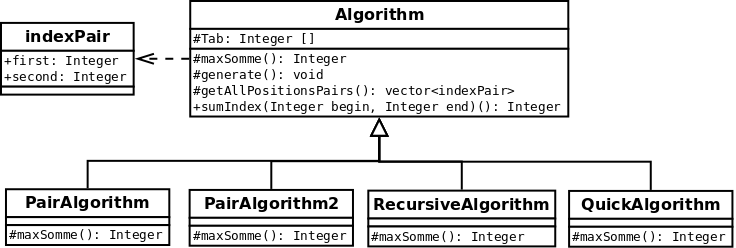
\includegraphics[scale=0.3]{diagramme.png}
	\caption{Diagramme UML du programme}
	\label{uml}	
\end{figure}

 
Les algorithmes implémentés doivent calculer la différence entre deux cases du tableau. J'ai décidé de créer une structure très simple, appelée IndexPair, contenant deux entiers: first et second, contenant chacun une cellule du tableau:
\begin{verbatim}
struct {
    int first;
    int second;
}
\end{verbatim}

\subsection{Méthodes principales}
Voici les méthodes, ainsi que leurs complexités respectives, qui sont implémentées dans la classe mère pour être ensuite réutilisées dans tous les algorithmes.
\subsubsection{Méthode: generate(Int n): void}
Cette méthode remplit le tableau avec des nombres aléatoires entre -1000 et 1000. Le paramètre $n$ correspond au nombre de cases désirées pour le tableau, et l'algorithme est très simple:
\begin{verbatim}
Pour i allant de 1 à n:
    tab[i] = random(-1000, 1000)
FinPour
\end{verbatim}
La complexité de la fonction random étant constante, cette méthode a une complexité en $\theta (n)$.

\subsubsection{Méthode: getAllPositionPairs()}
Cette méthode calcule toutes les paires possibles en fonction de la taille du tableau. Par exemple pour un tableau [1, 2, 3, 4], elle renverra un tableau qui contient les paires {[1,2], [1, 3], [1, 4], [2, 3], [2, 4], [3, 4]}
L'algorithme est le suivant:
\begin{verbatim}
Paires = []
Pour i allant de 1 à n-1:
    Pour j allant de i+1 à n:
        Paires.ajouter([i, j])
    FinPour
FinPour
\end{verbatim}
Cet algorithme est assez simple à implémenter, et nécessaire pour plusieurs des algorithmes de MaxSomme. Sa complexité est en $\theta (n^2)$.
\subsubsection{Méthode: sumIndex(Int a, Int b): int}
\section{Algorithme 1 : PairAlgorithm}
\subsection{Implémentation}

\end{document}